
Zu Beginn wurden Messungen direkt an dem Prozessor durchgeführt, um zu kontrollieren, dass die im Programm errechneten Signale auch die vorgesehenen Frequenzen erreichen. Anschließend wurden einzelne Baugruppen mit dem Prozessor kombiniert, um das Zusammenspiel dieser auswerten zu können. Danach wurden die Baugruppen um den Sensor erweitert und auch dieses Zusammenspiel wurde ausgewertet. Zum Abschluss wurde dann die komplette Platine im Betrieb getestet und optimiert.

\section{PWM-Ausgabe}
Um das Signal für die Entfernungsmessung zu generieren wurde der Mikrocontroller so programmiert, dass zehn Impulse mit einer Frequenz von 40kHz ausgegeben werden. Danach erfolgt eine Pause, um das zurückkehrende Signal abzuwarten und auszuwerten.\\
\begin{figure}[H]
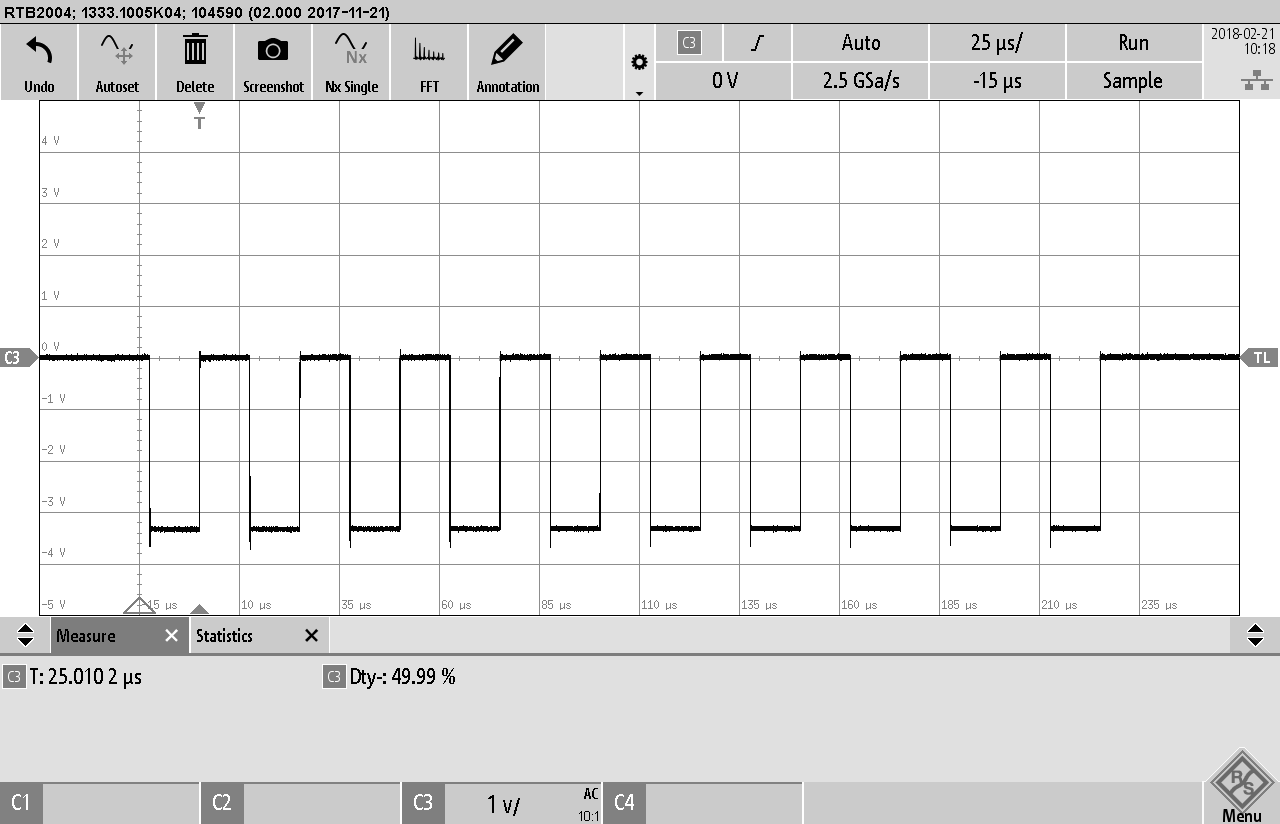
\includegraphics[width=1.0\textwidth]{Abbildungen/PWM-Signal.png}\caption{PWM-Burst auf 40kHz Basis}\label{fig:pwm-burst}
\end{figure}
In der Abbildung \ref{fig:pwm-burst} ist zu sehen, dass ein Burst aus zehn Impulsen mit einer Periodendauer von jeweils 25us generiert wurde. Diese Messung wurde direkt an dem Mikrocontroller vorgenommen, um sicherzustellen dass die H-Brücke mit der passenden Frequenz angesteuert wird.
\begin{figure}[H]
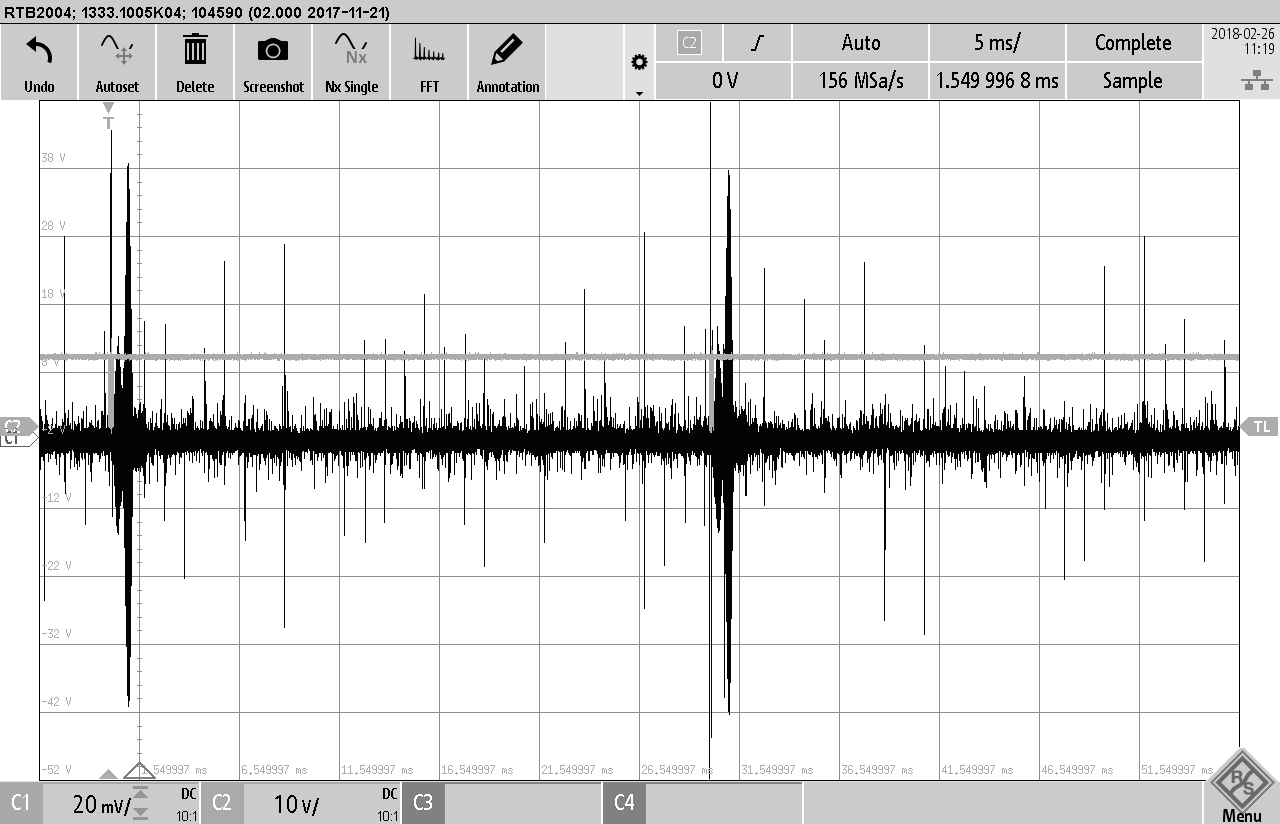
\includegraphics[width=1.0\textwidth]{Abbildungen/Abstand1.png}\caption{Versuchsmessung mit Sender und Empfänger parallel}\label{fig:Abstand1}
\end{figure}
In der Abbildung \ref{Abstand1} ist zu sehen, wie das Eingangssignal am Empfänger aussieht, wenn der Sender und der Empfänger getrennt aufgebaut sind und parallel auf ein Hinderniss gerichtet sind. Dabei zeigt die graue Linie den Verlauf des Sendersignals und die schwarze Linie den Verlauf des Empfängersignals
\section{H-Brücke}
Mach ersten Versuchen wurde die H-Brücke durch einen IXDN602, einen MOSFET ersetzt. Dies geschah, weil erstens die Beschaltung des OPV nur für eine positive Halbwelle funktioniert und zweitens die Beschaltung der H-Brücke fehlerhaft war. So wurde einer der Ausgänge auf Masse gelegt, was im Betrieb einen Kurzschluss verursachen würde. Um diese Probleme zu beheben, müssten der Sender- und der Empfängerkreis aufgetrennt werden und eine zweite Ultrashallkapsel eingesetzt werden. Dadurch ließ sich eine Reihe an Tests an der Senderschaltung durchführen. Allerdings viel auf, dass im Betrieb keine Signale empfangen wurden. Der Grund dafür war, dass der Mosfet als Low-Side-Driver geschaltet war, was bedeutet dass er das Signal entweder auf High, oder auf Low zieht. Somit werden auch alle von der Ultraschallkapsel empfangenen Signale direkt auf Low gezogen. Also musste eine weitere Überlegung angestellt werden und es wurden aus einem Mosfet zwei. Einer, der vom Prozessor angesteuert wird(3.3V) und den zweiten, der die Sendespannung(5V-20V) freigibt, schaltet. 

\section{Signalverlauf nach Verstärkung durch den OPV}
Durch die Verbindung der Sender- und der Empfängerseite entstand das Problem, dass die Entstörkondensatoren am Empfänger durch den Sendebetrieb zu sehr aufgeladen wurden, und sich danach erstmal entladen mussten, was eine Spannung am Sender/Empfänger zur Folge hatte. Das Entladen der Kondensatoren dauerte länger als die Pausen zwischen den Sendeimpulsen, dadurch konnten keine Signale empfangen werden.Um dieses Problem zu beheben wurde versucht, die OPV's durch einen MOSFET vom Sensor zu trennen, so lange gesendet wird. Da dieses erfolglos blieb wurde der Empfänger durch eine weitere Filterstufe erweitert.
